% \begin{appendices}
\appendix 
\section{Apêndice - Gráficos com total de área perdida ano a ano por estado}

\hspace{13pt} Os gráficos a seguir mostram os anos que mais houveram perda de área para cada estado presente no bioma. O valor da área está em metros quadrados. Todos os gráficos apresentados se referem apenas a eventos com duração igual a um ano, ou seja, não incluem dados referentes a eventos longos de degradação. Essa escolha se deu devido a grande presentação de eventos de longa duração no primeiro ano da análise, o que torna difícil e pouco interessante a análise dos gráficos.

\begin{figure}[H]
    \centering
    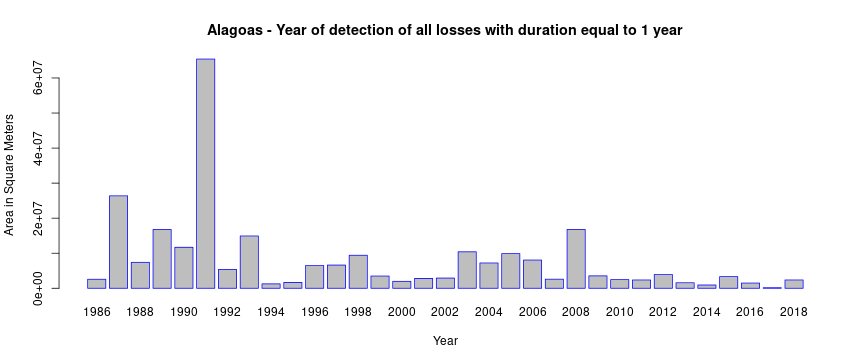
\includegraphics[scale=.5]{images/loss_graphics/Alagoas_loss_eq1.png}
    \caption{Perda de área por ano em Alagoas}
    \label{fig:loss_alagoas}
\end{figure}

\begin{figure}[H]
    \centering
    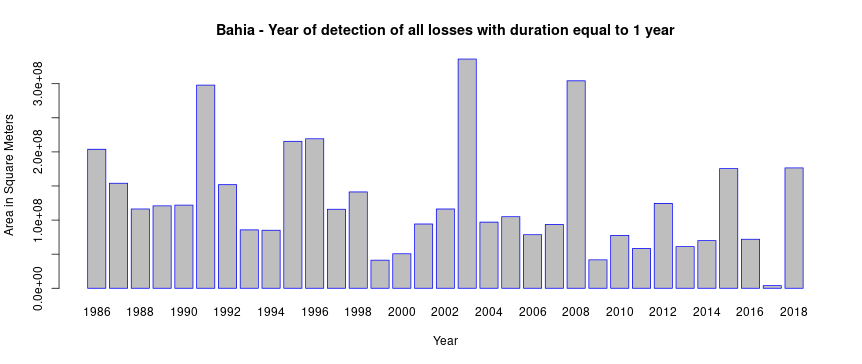
\includegraphics[scale=.5]{images/loss_graphics/Bahia_loss_eq1.png}
    \caption{Perda de área por ano na Bahia}
    \label{fig:loss_bahia}
\end{figure}

\begin{figure}[H]
    \centering
    \includegraphics[scale=.5]{images/loss_graphics/Espírito Santo_loss_eq1.png}
    \caption{Perda de área por ano no Espírito Santo}
    \label{fig:loss_espirito_santo}
\end{figure}

\begin{figure}[H]
    \centering
    \includegraphics[scale=.5]{images/loss_graphics/Goiás_loss_eq1.png}
    \caption{Perda de área por ano em Goiás}
    \label{fig:loss_goias}
\end{figure}

\begin{figure}[H]
    \centering
    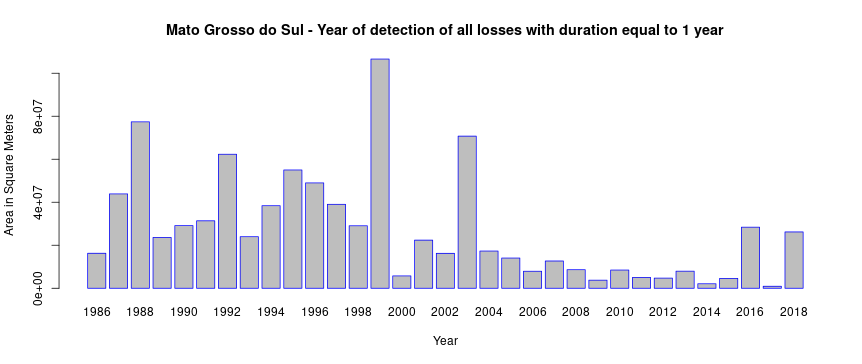
\includegraphics[scale=.5]{images/loss_graphics/Mato Grosso do Sul_loss_eq1.png}
    \caption{Perda de área por ano no Mato Grosso do Sul}
    \label{fig:loss_mato_grosso_sul}
\end{figure}

\begin{figure}[H]
    \centering
    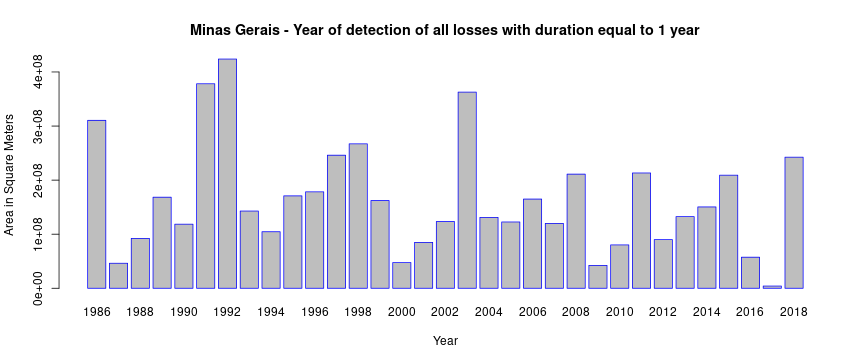
\includegraphics[scale=.5]{images/loss_graphics/Minas Gerais_loss_eq1.png}
    \caption{Perda de área por ano em Minas Gerais}
    \label{fig:loss_minas_gerais}
\end{figure}

\begin{figure}[H]
    \centering
    \includegraphics[scale=.5]{images/loss_graphics/Paraíba_loss_eq1.png}
    \caption{Perda de área por ano na Paraíba}
    \label{fig:loss_paraiba}
\end{figure}

\begin{figure}[H]
    \centering
    \includegraphics[scale=.5]{images/loss_graphics/Paraná_loss_eq1.png}
    \caption{Perda de área por ano no Paraná}
    \label{fig:loss_parana}
\end{figure}

\begin{figure}[H]
    \centering
    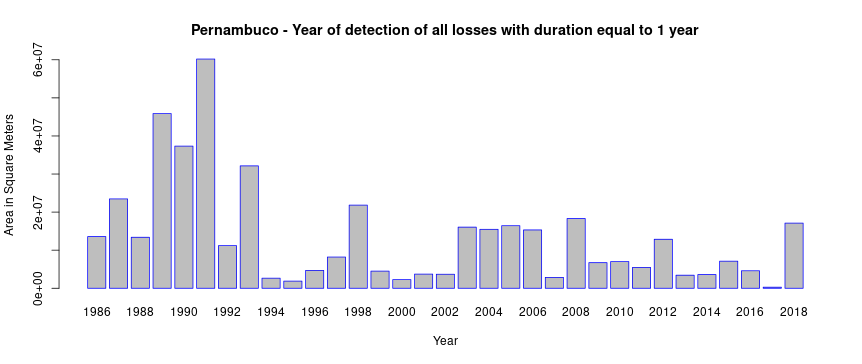
\includegraphics[scale=.5]{images/loss_graphics/Pernambuco_loss_eq1.png}
    \caption{Perda de área por ano em Pernambuco}
    \label{fig:loss_pernambuco}
\end{figure}

\begin{figure}[H]
    \centering
    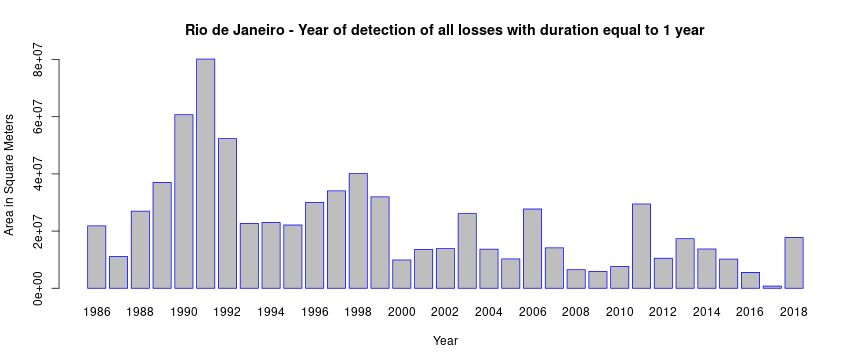
\includegraphics[scale=.5]{images/loss_graphics/Rio de Janeiro_loss_eq1.png}
    \caption{Perda de área por ano no Rio de Janeiro}
    \label{fig:loss_rio_de_janeiro}
\end{figure}

\begin{figure}[H]
    \centering
    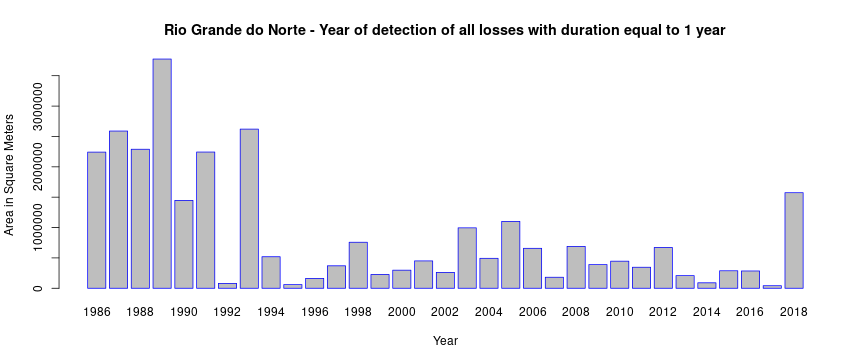
\includegraphics[scale=.5]{images/loss_graphics/Rio Grande do Norte_loss_eq1.png}
    \caption{Perda de área por ano no Rio Grande do Norte}
    \label{fig:loss_rio_grande_do_norte}
\end{figure}

\begin{figure}[H]
    \centering
    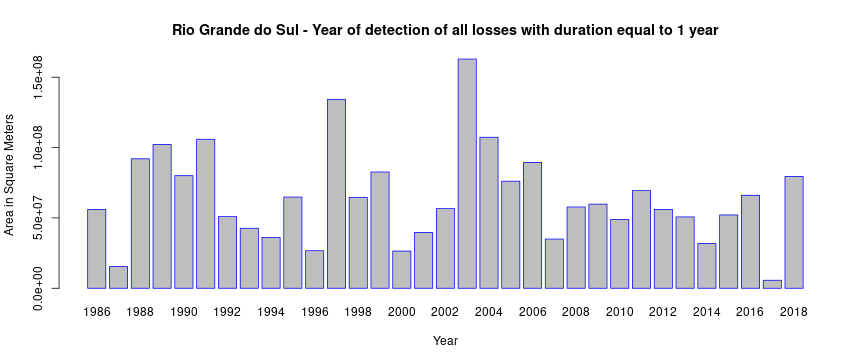
\includegraphics[scale=.5]{images/loss_graphics/Rio Grande do Sul_loss_eq1.png}
    \caption{Perda de área por ano no Rio Grande do Sul}
    \label{fig:loss_rio_grande_do_sul}
\end{figure}

\begin{figure}[H]
    \centering
    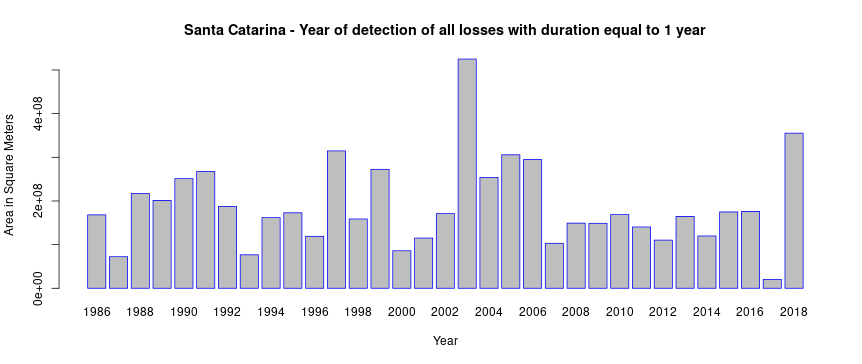
\includegraphics[scale=.5]{images/loss_graphics/Santa Catarina_loss_eq1.png}
    \caption{Perda de área por ano em Santa Catarina}
    \label{fig:loss_santa_catarina}
\end{figure}

\begin{figure}[H]
    \centering
    \includegraphics[scale=.5]{images/loss_graphics/São Paulo_loss_eq1.png}
    \caption{Perda de área por ano em São Paulo}
    \label{fig:loss_sao_paulo}
\end{figure}

\begin{figure}[H]
    \centering
    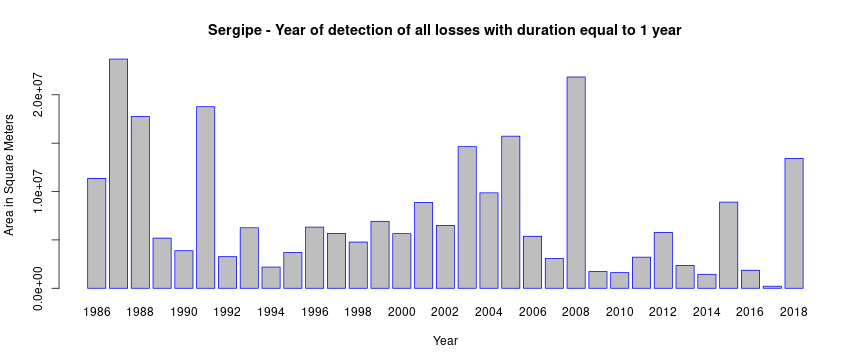
\includegraphics[scale=.5]{images/loss_graphics/Sergipe_loss_eq1.png}
    \caption{Perda de área por ano em Sergipe}
    \label{fig:loss_sergipe}
\end{figure}

% \end{appendices}